\chapter{Reporting}\label{sec:Reporting}
Reporting is a core concept of Varroa.
Its purpose is determine the result values of a Varroa test and output them in a verifiable document.
For that reason there are entities that observe the parts of Varroa that execute the scenario.
These exist on different hierarchy levels.
Figure \ref{fig:ReportingArchitecture} shows the entities that are responsible for observing the actions that have taken place as well as their hierarchy.

\section{Reporting Architecture}
\begin{figure}[H]
	\begin{center}
		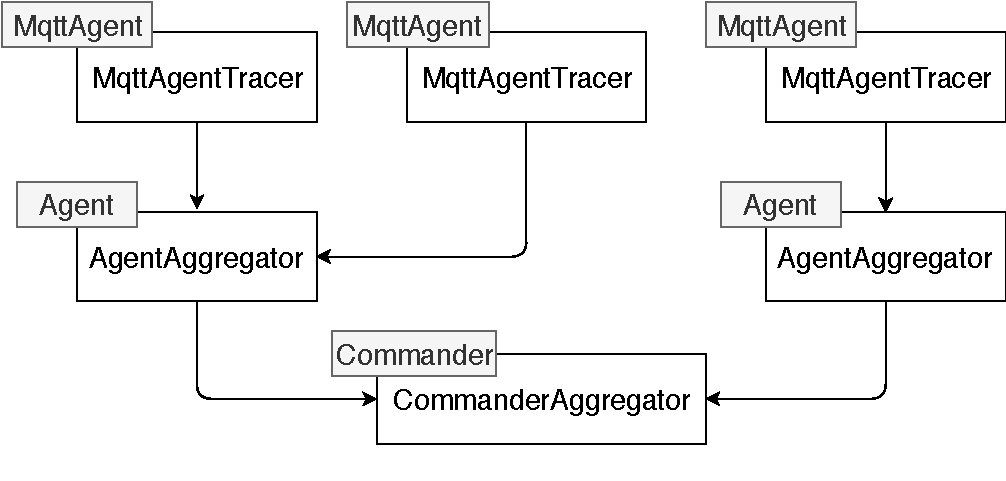
\includegraphics[scale=0.75]{Resources/PDF/ReportingArchitecture}
		\caption{Reporting Architecture}
		\label{fig:ReportingArchitecture}
	\end{center}
\end{figure}
The reporting architecture is organized in strong accordance to Varroas hierarchy.
The data flow of the report happens bottom up from the Agents to the Commander.
The reported data is recorded at the lowest level of the hierarchy namely the \emph{MqttAgentTracer} which tracks its MqttAgents' Actions.
Subsequently the \emph{AgentAggregator} receives this data and aggregates it before passing the result to the Commander.
The CommanderAggregator collects the received data 
and then aggregates the whole information of all Agents and compiles it into the report.
Figure \ref{fig:ReportingArchitecture} visualizes the realitationships between the components explained above.

\section{Metrics}
\begin{lstlisting}[caption={Reporting Output}, captionpos=, label={lst:ReportingOutput}, language=]
1=ActionReport{
	durationSampler=[count=50, mean=146ms, stdDev=139ms, min=39ms, max=694ms], latenessSampler=[count=31, mean=118ms, stdDev=155ms, min=1ms, max=614ms]
};
\end{lstlisting}
Listing \ref{lst:ReportingOutput} shows an excerpt from a reporting output.
The Number at the beginning references the Command this ActionReport corresponds to in the order they are defined in the Scenario.
\subsection{Duration Sampler}
The Duration Sampler gives metrics based on the duration of the executed Actions:
\begin{itemize}
	\item \textbf{count:} the amount of executed Actions.
	\item \textbf{mean:} the mean duration of the executed Actions.
	\item \textbf{stdDev:} the standard deviation of the duration of the executed Actions.
	\item \textbf{min:} the minimum duration of the executed Actions.
	\item \textbf{max:} the maximum duration of the executed Actions.
\end{itemize}
\subsection{Lateness Sampler}
The Duration Sampler reports metrics based on the overruning of expected durations of the executed Actions:
\begin{itemize}
	\item \textbf{count:} the amount of Actions whose durations exeeded the expected duration.
	\item \textbf{mean:} the mean lateness value of the actions.
	\item \textbf{stdDev:} the standard deviation of the executed Actions lateness.
	\item \textbf{min:} the minium lateness of the executed Actions.
	\item \textbf{max:} the maximum lateness of the executed Actions.
\end{itemize}

\subsection{Failed Count}
%TODO

